%%%%%%%%%%%%%%%%%%%%%%%%%%%%%%%%%%%%%%%%%%%%%%%%%%%
%
%  New template code for TAMU Theses and Dissertations starting Fall 2016.  
%
%
%  Author: Sean Zachary Roberson
%  Version 3.17.09
%  Last Updated: 9/21/2017
%
%%%%%%%%%%%%%%%%%%%%%%%%%%%%%%%%%%%%%%%%%%%%%%%%%%%
%%%%%%%%%%%%%%%%%%%%%%%%%%%%%%%%%%%%%%%%%%%%%%%%%%%%%%%%%%%%%%%%%%%%%%
%%                           SECTION IV
%%%%%%%%%%%%%%%%%%%%%%%%%%%%%%%%%%%%%%%%%%%%%%%%%%%%%%%%%%%%%%%%%%%%%



\chapter{EVENT RECONSTRUCTION \label{cha:eventreco}}
In the CMS detector, collisions happen in a small longitudinal region near the center called the luminous region or interaction region. Collisions themselves are not recorded, only the particles that get created. The origin of one or more new particles is called a vertex. An event is the set of particle measurements in the detector associated to a single beam-beam crossing. It is the job of the reconstruction software to process the raw information and identify physics objects for a given event.

 \begin{figure}[H]
 	\centering
 	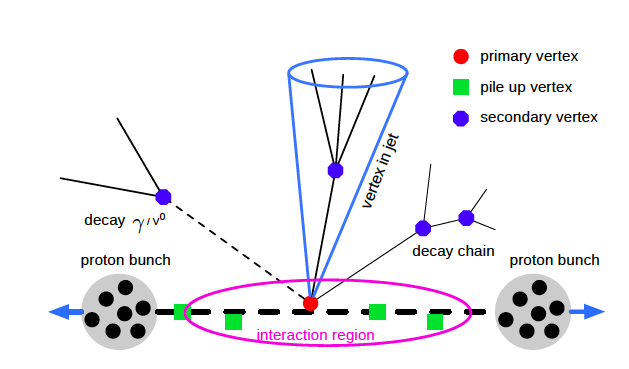
\includegraphics[width=0.75\textwidth]{figures/eventvertex.png}
 	\singlespace
 	\caption{Schematic diagram for an event at the LHC.}
 	\label{fig:vertex}
 \end{figure}


\section{Data Acquisition}
The CMS Data Acquisition (DAQ) and trigger system was specifically designed to collect and analyze data at a rate of 40MHz, which corresponds to a 25 ns collision rate. Unfortunately, due the electronics system is only able to record a few hundreds of Hz of events. Therefore, events are filtered online by so-called trigger systems, so that only interesting events are written to disk. The collision triggering the readout is called the primary vertex, while other collisions from the beams are called pile-up. Secondary vertices refer to the other production points, when particles are created from decay or hard-scattering. This is shown in Figure \ref{fig:vertex}. Particles from the primary vertex usually have a high transverse momentum ($p_{T}$), making them interesting and easier to study.

\subsection{L1 Trigger and HLT}
 When CMS is performing at its peak, about one billion proton-proton interactions will take place every second inside the detector. In order to record only those events generated from energetic, head-on collisions, a "trigger" system was implemented.

Level 1 of the trigger is an extremely fast, hardware based process that looks for simple signs of interesting physics, e.g. particles with a large amount of energy or in unusual combinations. The L1 trigger selects events at a rate of around 100 kHz within a time interval of 4$\mu$s. The next step is the HLT, which combines the information from different parts of the detector to recreate the entire event and send it to a farm of more than 1000 computers to filter even more events, reducing the event rate to less than 1 kHz before recording them on tape.

\subsection{T1 sites and data storage}

CMS computing operates on a tiered computing structure. A Tier-0 computing center is located at CERN where the data is transferred form the HLT and a first set of reconstruction occurs. From there, it is transferred to one of seven Tier-1 computing centers located around the world. At the Tier-1 centers, a full reconstruction of the data is performed. Furthermore, there are 55 Tier-2 centers which can be accessed by the collaboration members for data processing and storage.

 \begin{figure}[H]
 	\centering
 	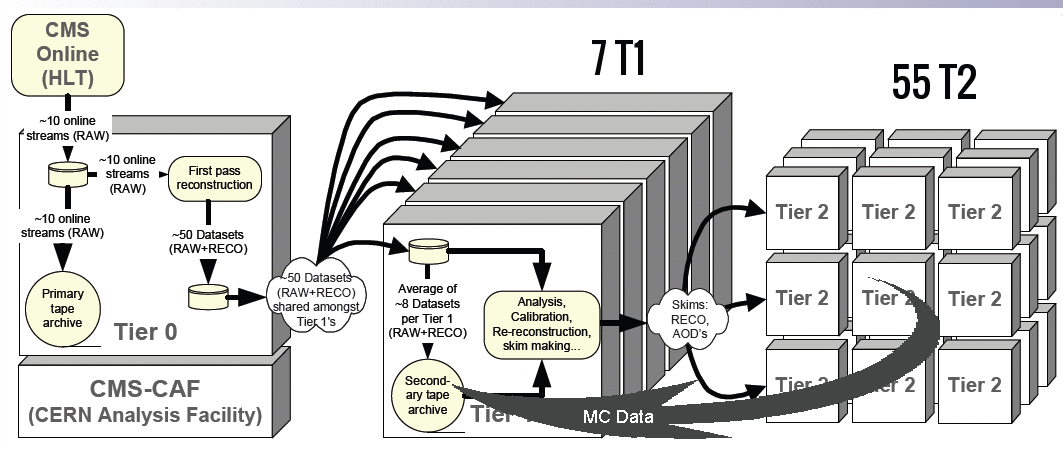
\includegraphics[width=0.75\textwidth]{figures/dataflowtiers_MC.png}
 	\singlespace
 	\caption{Flow of CMS detector data through the tiers. Reprinted from \cite{CMSdatatier}}
 	\label{fig:datatier}
 \end{figure}

 The data itself is also processed in three data tiers. The first layer of this is the RAW data, which is created by unpacking detector streams passed on from the L1 and HLT triggers, typically composed of measurements from the different calorimeters as well as some information provided by the L1 trigger. This RAW data is reconstructed into physics objects(i.e. muons, electrons, photons) that can be grouped later for further analysis. This step is called RECO, which is short for reconstruction and contains both the detector and physics object information. 

 After RECO, an \textit{analysis object data} (AOD) is formed from a subset of the RECO information. AOD objects are typically comprised of only high-level physics objects, making the files much smaller. This data format is usually the preferred one for physics analysis.



\section{Particle Flow Event Reconstruction}
\label{sec:track}

As mentioned in Section 2, CMS is one of the two general-purpose detectors at the LHC, and as such, it was designed based on the concept of cylindrical detection layers. In the previous section we described how data was managed and stored during the acquisition process. This section will focus on how physicists make sense of the raw detector information.  

 First, detector data is measured in the form of electronic signals, i.e. hits in the tracker or energy depositions in the calorimeters. Then, the trajectories of charged particles, or tracks, are reconstructed from the position hits in the detector. From the collection of tracks in an event, the primary and any secondary vertices are reconstructed. 

An optimal event description can be achieved by correlating the basic elements from all detector layers (tracks and clusters) to identify each final-state particle, and by combining the corresponding measurements to reconstruct the particle properties on the basis of this identification. At CMS, this approached is called \textit{particle-flow (PF) reconstruction}.

The reconstructed and identified individual particle list includes muons, electrons, photons, charged hadrons, as well as stable and unstable neutral hadrons. These particles can be non-isolated, and even originate from an intricate overlap of reconstructed charged particles, ECAL and HCAL energy clusters, and signals in the muon chambers.

Looking at Figure \ref{fig:cmsslice}, one can see that photons and neutral hadrons are in general identified by ECAL and HCAL clusters with no track link. No attempt is made to distinguish the various species of neutral and charged hadrons in the PF reconstruction. Electrons can be identified by a track and an ECAL cluster, with a momentum-to-energy ratio compatible with unity, and not connected to an HCAL cluster. Finally, muons and neutrinos would traverse the calorimeters with little or no interactions. While neutrinos would escape undetected, muons would be identified by a track in the inner tracker connected to a track in the muon detectors.

 \begin{figure}[h]
  	\label{fig:cmsslice}
 	\centering
 	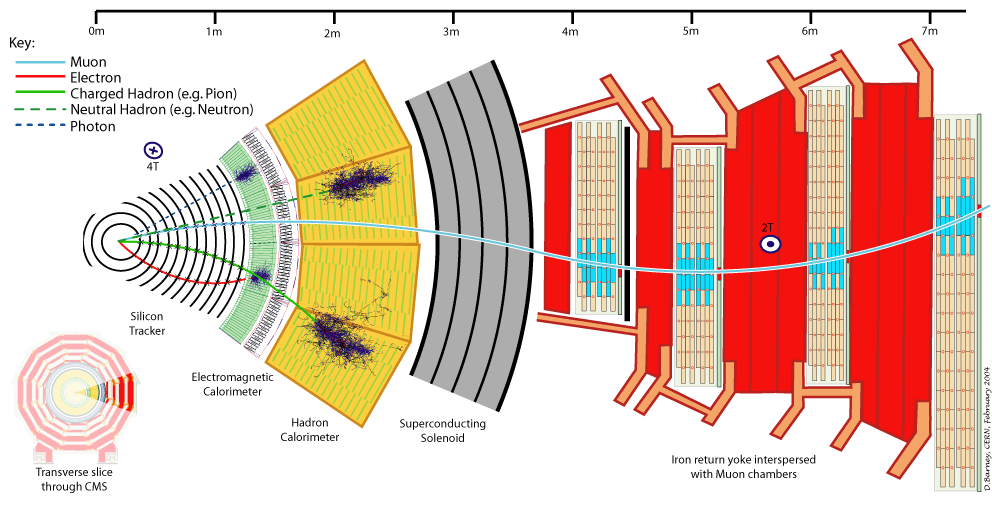
\includegraphics[width=0.75\textwidth]{figures/image005.png}
 	\singlespace
 	\caption{Cross-sectional view of the CMS detector with all of the sub-detectors labeled. The colored lines correspond to different particle types. Each particle interacts with different pieces of the detector and may or may not be bent by the magnetic field. Reprinted from \cite{CMSSlice}}
 \end{figure}

The PF concept was developed and used for the first time by the ALEPH experiment at LEP\cite{BUSKULIC1995481} and can now be used in hadron colliders due to the very fine spatial granularity of the detectors. In particular, CMS is very well suited for PF reconstruction due to its highly-segmented tracker,  a fine-grained ECAL, and an hermetic HCAL.

Also, the CMS magnet is large enough to accommodate the tracker and both the ECAL and HCAL, thereby minimizing the mount of material in front of the calorimeters. This particular feature is an advantage for PF reconstruction, as it eliminates the energy losses before the calorimeters caused by particles showering in the coil material and facilitates the link between tracks and calorimeter clusters.

\subsection{Iterative Tracking}

 The first step of the reconstruction process is referred to as local reconstruction and it consists of the clustering of \textit{zero-suppressed} signals above specified thresholds in pixel and strip channels into hits. The next step is track reconstruction, which refers to the process of using the reconstructed hits to obtain estimates for the momentum and position parameters of the charged particles responsible for the detector hits. 

 The tracking software at CMS\cite{TRK-11-001} is commonly referred to as the combinatorial Track Finder (CTF), which is an adaptation of the combinatorial Kalman Filter \cite{Billoir:1989mh},\cite{BILLOIR1990219},\cite{Mankel:1997dy}, which in turn is an extension of the Kalman filter\cite{Fruhwirth:1987fm} to allow pattern recognition and track fitting to occur in the same framework. The collection of reconstructed tracks is produced by multiple passes or iterations of the same CTF track reconstruction sequence, in a process called iterative tracking. 

The basic idea of iterative tracking is that the initial iteration seach for tracks that are easiest to find (e.g., of relatively large $p_{T}$, and produced near the interaction region). After each iteration, hits associated with tracks are removed, thereby reducing the combinatorial complexity, and simplifying subsequent iterations in a seach for more difficult classes of tracks (e.g., low $p_{T}$, or greatly displaced tracks).

Each iteration proceeds in four steps:

\begin{itemize}
	\item Seed generation which provides track candidates consisting of a few (2 or 3) hits. Seeds are generated in the innermost layers of the tracker and are commonly referred to as "proto-tracks".
	\item Track finding, which is based on a Kalman filter. It extrapolates the seed trajectories along the expected flight path of a charged particle, searching for additional hits that can be assigned to the track candidate.
	\item Track fitting. A module that is used to provide the best possible estimate of the parameters of each trajectory by means of a Kalman filter.
	\item Track selection. This step sets the quality flags and discards tracks that fails certain specified criteria.
\end{itemize}

A total of six iterations are used, each with different seed generation, $p_{T}$ and impact parameter requirements.

The first iterations have strict criteria in order to achieve a negligible small fake rate. Once the hits are associated with these tracks are removed, the seeding criteria is loosened. By doing this, tracking efficiency is increased. From iteration 4 and on, the constraints on the tracks closer to the interaction point are slowly relaxed. This allows for reconstruction of secondary charged particles created from photon conversions and nuclear interactions in the tracker volume.

\subsection{Calorimeter Clustering}
Clustering in the calorimeters is the process of grouping detector cells that register hits together to measure the energy and direction of stable neutral particles. Additionally, clustering seeks to separate the neutral particles from energy deposits associated with charged hadrons, reconstruct electrons (including all associated Bremsstrahlung photons), and measure the energy of charged hadrons for which tracks were not determined accurately. The clustering algorithm is performed separately in each sub-detector: ECAL barrel and endcap, HCAL barrel and endcap, and in the pre-shower.

The clustering proceeds via three steps\cite{CMS:2009nxa}:

\begin{enumerate}
	\item Identify 'cluster seeds'. These are defined as the cell in a calorimeter with a local maximum of energy (above some set threshold).
	\item Expand from the seed to grow 'topological clusters'. This is done by aggregating calorimeter cells that have at least one side in common with the seed cell, and also have an energy over a particular threshold.
	\item Repeat the process of cluster growing, now using new cells that are part of the cluster.
\end{enumerate}

In this sense, a "seed" gives rise to a "particle-flow cluster". If a cell is identified by two clusters, the energy is shared between the clusters according to the distance from the cell to the center of each cluster. The cluster energies and positions are iteratively determined as new cells are added to the cluster.

\subsection{Linking Tracks and Clusters}
Once the basic PF elements like the trajectories of charged particles in the inner tracker, electron and muon tracks, and calorimeter clusters are available, the next step in reconstructing a particle is the so-called \textit{link algorithm}.

 The link algorithm can test any pair of elements in the event. In order to prevent the computing time of the link algorithm from growing quadratically with the number of particles, the pairs of elements considered by the link procedure are restricted to the nearest neighbors in the ($\eta,\phi$) plane, as obtained with a $k$-dimensional tree\cite{Bentley1975MultidimensionalBS}. The specific conditions required to link two elements depend on their nature.

 If two elements are found to be linked, the algorithm defines a distance between these two elements, aimed at quantifying the quality of the link. The link algorithm then produces \textit{PF blocks} of elements associated either by a direct link or by an indirect link through common elements.

 The link between tracks and calorimeter clusters proceeds by extrapolating the last measured hit in the tracker to one of the three detectors\cite{CMS:2009nxa}:

 \begin{itemize}
 	\item The two layers of the pre-shower detector,
 	\item the ECAL, at a depth corresponding to the expected maximum of the electron shower profile,
 	\item the HCAL, to a depth corresponding to one interaction length.
 \end{itemize}

 The track is then linked to a cluster in these detectors if the extrapolated position is within the cluster boundaries. Additionally, to link Bremsstrahlung photons to their associated electron, tangents to the track are extrapolated to the ECAL and cluster found within those boundaries is also linked.

 Similarly, links between the calorimeters are formed when a cluster from the more granular calorimeter (pre-shower or ECAL) is within the cluster envelope of the less granular calorimeter (ECAL or HCAL).

 Finally, muon tracks are linked to charged particle tracks by a global fit between the two sets of tracks.

 \section{Physics Object Reconstruction}

With the tracks identified, calorimeter clusters formed and the linking of clusters to tracks, particles can then be reconstructed. The particle flow process begins by reconstructing muons, then electrons and photons, and finally charged hadrons. As each particle is reconstructed, the tracks and clusters associated with it are removed from the collection of blocks used to form candidate particles, which ensures that energy deposits attributed to one particle are not used twice. The hadrons are then clustered together to form jets, and these jets can additionally be identified as coming from tau leptons or b quarks (Figure \ref{fig:pf}).


 \begin{figure}[h]
  	\label{fig:pf}
 	\centering
 	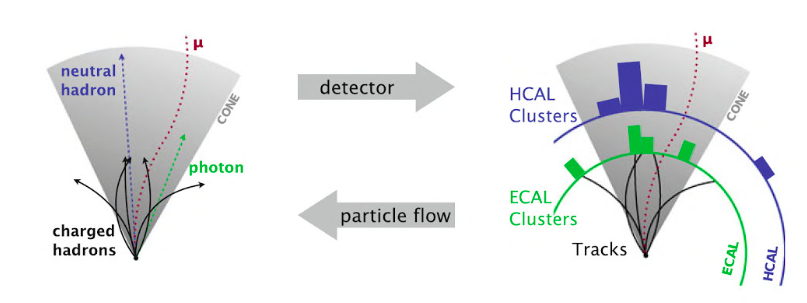
\includegraphics[width=0.75\textwidth]{figures/jets.png}
 	\singlespace
 	\caption{CMS Particle Flow algorithm. The diagram shows how collisions lead to particle decays and final state particles. On the right side of the diagram the tracks and deposits in the CMS detector are shown. The left side shows that PF candidates are derived from detector information and then become input for the PF algorithm that uses them to construct high-level physics objects like electrons, which are then used by analysts to reconstruct the collision event. Reprinted from \cite{CMS-PAS-PFT-09-001}}
 \end{figure}

\section{Jets}

During proton-proton collisions, the confined state of quarks and gluons is broken. This de-confined state of the free partons does not last very long, as it is not allowed by QCD. Shortly after the collision, partons hadronize and a bunch of particles is generated by this process. These particles are usually collimated in a given direction due to the boosted nature of the parton, and thereby producing a jet or spray of particles around it.

\begin{figure}[h]
  	\label{fig:jets2}
 	\centering
 	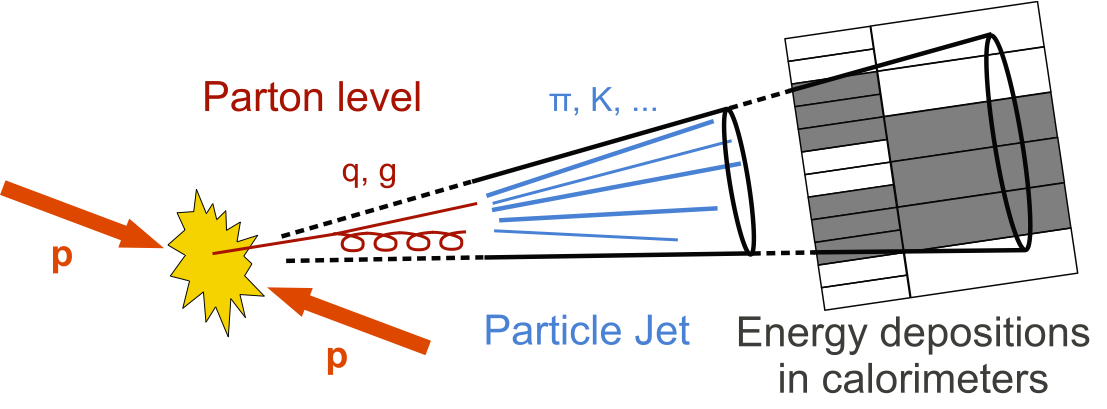
\includegraphics[width=0.75\textwidth]{figures/jetsatcmsand.png}
 	\singlespace
 	\caption{Diagram of proton-proton collision producing a jet}
 \end{figure}

In practice, jets are the result of clustering groups of charged hadrons, photons, and neutral hadrons coming from PF. The energy fraction in jets is divided amongst them with a breakdown of roughly 65$\%$, 25$\%$, and 10$\%$ respectively. This is illustrated in Figure \ref{fig:jme}. For this study, jets were reconstructed from PF candidates clusters using the anti-$k_{T}$ algorithm\cite{Cacciari:2008gp} as defined in the FASTJET package\cite{Cacciari:2011ma}.

\begin{figure}[h]
  	\label{fig:jme}
 	\centering
 	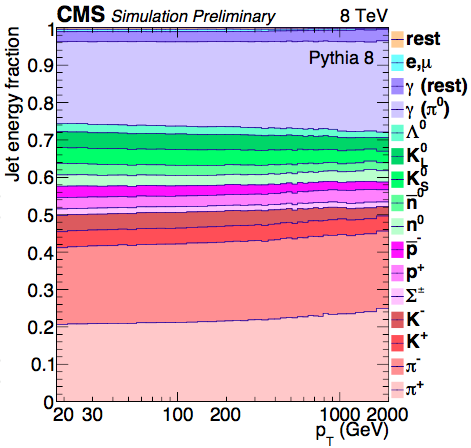
\includegraphics[width=0.75\textwidth]{figures/jme.png}
 	\singlespace
 	\caption{Jet composition}
 \end{figure}

 Jet clustering algorithms work by defining a distance parameter($d_{ij}$) between to PF candidates $i$ and $j$, and the distance between such cluster and the beam, $d_{iB}$. These are defined as

 \begin{align}
 \label{jetclust}
 d_{ij} = min(k_{ti}^{2p},k_{tj}^{2p})\frac{\Delta_{ij}^{2}}{R^{2}}
 d_{iB} &= k_{ti}^{2p}
 \end{align}

where $\Delta_{ij}^{2} = (y_{i}-y_{j})^{2}+(\phi_{i}-\phi_{j})^{2}$, and $k_{ti}$, $y_{i}$, and $\phi_{i}$ are the transverse momentum, rapidity, and azimuth of particle $i$, respectively. R is a user-defined radius parameter, and $p$ is a measure of the relative power of energy vs geometric scales. Particularly, for the anti-$k_{T}$ algorithm, $p=-1$, and Equation \ref{jetclust} reduces to

\begin{equation}
d_{ij} = min(\frac{1}{p_{ti}^{2}},\frac{1}{p_{tj}^{2}})\frac{\Delta_{ij}^{2}}{R^{2}}
\end{equation}

The algorithm loops over all PF candidate objects, calculating $d_{ij}$ for each pair of objects. Once it does this, it selects the two objects with the lowest value of $d_{ij}$ and combines them. This process is repeated until the smallest value of $d_{ij}>d_{iB}$ for all the remaining pairs. 

As a result, the cutoff limit of $1/p_{T}^{2}$ defines a maximum size that the algorithm will look to cluster particles inside. The construction of $d_{ij}$ using the inverse $p_{T}^{2}$ has a result of producing values of $d_{ij}$ that are smaller for objects with a higher $p_{T}$, given equal separation. As a result, softer particles will tend to cluster to higher $p_{T}$ particles long before they would cluster amongst themselves. If no hard particles are present, the jet object will simply cluster soft $p_{T}$ particles in a circle in an $\eta-\phi$ space of radius R.

The clustering of the anti-$k_{T}$ algorithm leads to jets with a large $p_{T}$ being reconstructed as perfect circles, while softer jets can have a more ambiguous shape. Figure \ref{fig:antikt} shows a display of the anti-$k_{T}$ algorithm for a distance parameter R=1. Notice that the green jet around $y=2$ and $\phi=5$ has a circular shape, while it deforms the smaller jet right next to it.

Finally, the anti-$k_{T}$ algorithm is both infrared and collinear safe. Infrared safety means that the jet clustering algorithm is insensitive to the emission of soft, wide angle particles. Under this condition, two jets would not be merge due to one of them producing a high-momentum particle between them. Collinear safety means that if there is a splitting which results in two parallel high-$p_{T}$ particles, a single jet is produced and the jet properties will not be different from a jet where this splitting did not occur. If the algorithm follows these two properties, it is referred to as being IRC safe.

\begin{figure}[h]
  	\label{fig:antikt}
 	\centering
 	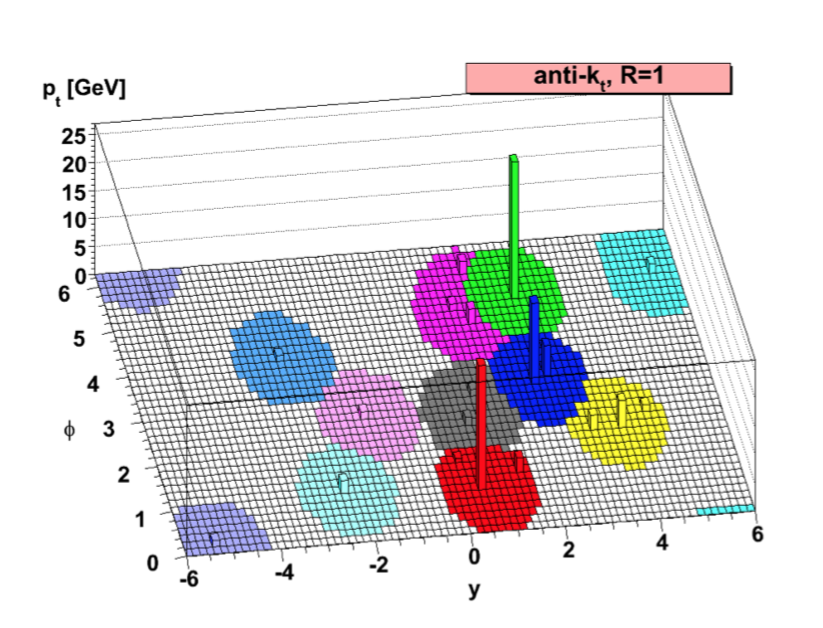
\includegraphics[width=0.75\textwidth]{figures/antikt.png}
 	\singlespace
 	\caption{A sample parton-level event clustered with the anti-$k_{T}$ algorithm. Reprinted from \cite{Cacciari:2008gp}}
 \end{figure}

The use of PF candidates, with their built in tracking information for jet reconstruction provides a jet resolution of 15$\%$ at 10 GeV, 8$\%$ at 100 GeV, and 4$\%$ at 1 TeV\cite{CMS-PAS-PFT-09-001}. 

After the clustering procedure, the momentum and energy of the reconstructed jets still might not be the same as those from the initial parton, whether because of additional pileup energy produced during the same bunch crossing as the primary vertex or detector effects. To correct for this, CMS adopted a factorized approach, where each level of correction targets a specific effect and each correction factor obtained is applied in order. The goal is to make sure each jet has a relative response

\begin{equation}
\mathcal{R}_{rel} = \frac{p_{T}^{reco}}{p_{T}^{ref}} 
\end{equation}

as close as possible to unity. Here $p_{T}^{reco}$ is the reconstructed jet $p_{T}$ and $p_{T}^{ref}$ is the true of reference $p_{T}$ of the jet. 

The process of correcting the jet 4-momentum by means of a scale or weight obtained from matching the reconstructed jet information to that of the reference jet in Monte Carlo is referred to as jet energy correction (JEC).

The first level of correction, commonly referred to as the L1FastJet corrections, starts by removing pileup or electronic noise energy that may have made it into the jet reconstruction. This multiplicative correction will only remove energy from within the jet and will take the form in Equation \ref{pileupeq}, where $\rho$ is the median energy density of the event, $A$ is the jet area, and $f$ is an estimate of the offset inside the jet per unit of jet area \cite{JINST2011,Cacciari2007}.

\begin{equation}
\label{pileupeq}
p_{T}^{L1Corrected} = p_{T}^{uncorrected}\dot(1 - A\frac{f(\eta,\rho,A)}{p_{T}^{uncorrected}})
\end{equation}

The L2Relative correction compensates for the non-linearity in the jet response as a function of $\eta$ while the L3Absolute correction does the same thing as a function of $p_{T}$. All three corrections are applied to both data and simulation. An additional level of correction, called L2L3Residual, is applied to data only in order to correct for the difference in scale between the data and simulation.

A final level of modification to the reconstructed objects is an $\eta$ dependent smearing factor applied to the jet 4-momenta coming from the MC samples. The distribution of jet energies within the MC simulation tends to be more sharply peaked and less broad than the same distribution in data, resulting in a smaller jet energy resolution (JER) than we can realistically measure using the CMS detector. The deterministic "smearing" method recommended by CMS matches the MC jet energy resolution to that in data. 

The reconstructed jet $p_{T}$ is scaled by a correction factor $C_{JER}$ as determined in Equation \ref{eq:C_JER}, where $C_{\eta}$ is a correction factor derived as a function of $\eta$. The multiplicative JER correction factor is then used to modify the jet 4-momentum as in Equation \ref{eq:Jet_JER}.

\begin{equation}
\label{eq:C_JER}
C_{JER}=max\left(0.0,\frac{p_{T}^{GEN}}{p_{T}^{RECO}}+C_{\eta}\cdot\left(1-\frac{p_{T}^{GEN}}{p_{T}^{RECO}}\right)\right)
\end{equation}

\begin{equation}
\label{eq:Jet_JER}
\textbf{X}_{Jet}^{corrected}=C_{JER}{\cdot}\textbf{X}_{Jet}^{RECO}
\end{equation}

A set of quality cuts, collectively called PF jet identification, are applied to the resulting collection of jets to ensure that only real, hard scatter PF jets are used during the analysis\cite{CMS-AN-2010-003}. Several working point are defined at varying levels of efficiency and purity, but this analysis makes use of the tight criteria shown in Table \ref{tab:PFJetID}\cite{PFJetID}.

\begin{table}[htbp]
    \caption{Cut based PF jet identification requirements for the tight working point.}
    \centering
    \begin{tabular}{llll}
        \hline
        \multirow{2}{*}{Cut Variable}               & Cut Value \\\cline{2-2}
                                                    & Tight\\ 
        \hline 
        $\eta$& $|\eta|<$2.7 &2.7$<|\eta|\leq$ 3.0  & $|\eta|>$ 3.0\\
        \hline 
        Neutral Hadron Fraction  & <0.90  & <0.98 & -\\  
        Neutral EM Fraction      & <0.90  & > 0.01 & <0.90\\
        $n_{constituents}$       & >1     & -      & - \\
        Muon fraction            & <0.8   & -      & -\\
        Number of Neutral Particles & - & > 2      & >10\\
        \hline
        and for $|\eta| \leq$ 2.4 in addition apply\\
        \hline
        Charged Hadron Fraction & > 0 \\
        Charged Multiplicity    & > 0 \\
        Charged EM Fraction     & < 0.90\\
        \hline 
    \end{tabular}
    \label{tab:PFJetID}
\end{table}

All cuts on the jet energy fractions are made on the raw jets, before any energy correction is applied. In addition to the PF jet quality cuts, this analysis requires that all jets be within |$\eta$| < 2.6 and to have a $p_{T} > $ 30 GeV. 

\section{b-tagging}
Some jets are produced from a b-quark that after hadronization gets transformed into a B meson that has a large lifetime, and subsequently decay after it has traveled some distance. B-tagging is the identification of jets at some confidence level as having decayed from a B meson.

\begin{figure}[h]
  	\label{fig:antikt}
 	\centering
 	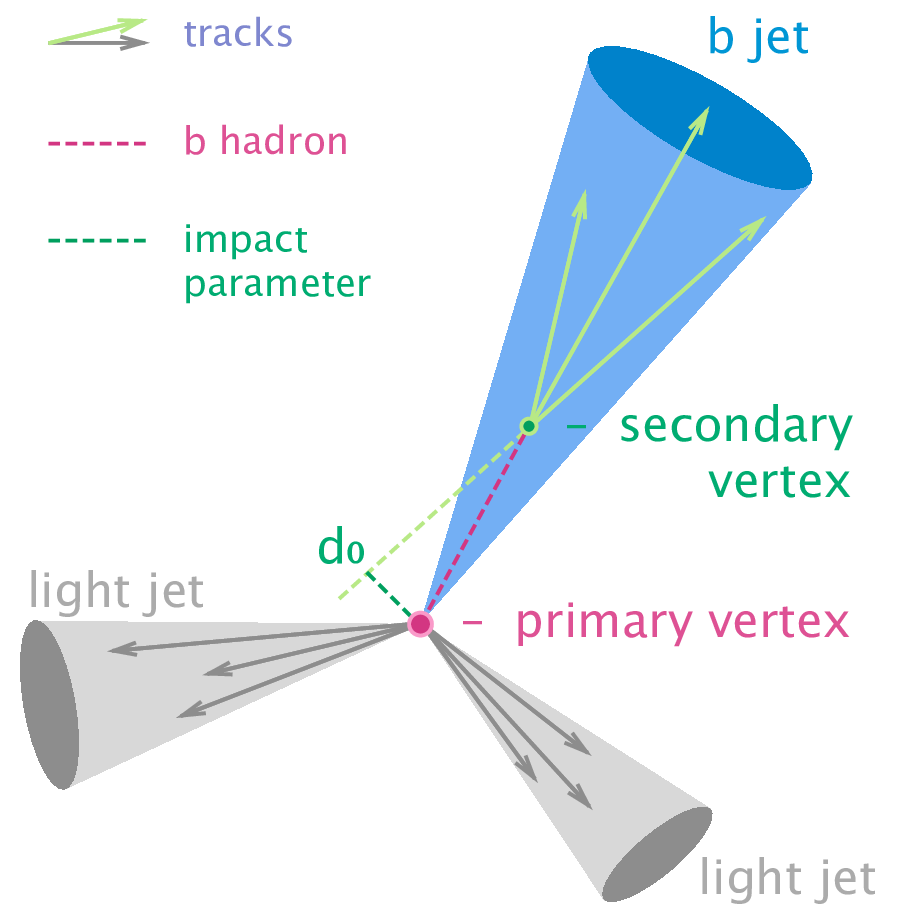
\includegraphics[width=0.75\textwidth]{figures/Btag.png}
 	\singlespace
 	\caption{Diagram showing the common principle of identification of jets initiated by B hadron decays. Reprinted from \cite{wiki:btag}}
 \end{figure}

A variety of b-tagging algorithms has been developed by CMS to select b-quark jets\cite{BTV-12-001} based on variables such as the impact parameters of the charged-particle tracks, the properties of reconstructed decay vertices, and he presence or absence of a lepton, or combinations thereof. These algorithms heavily rely on machine learning tools and are thus natural candidates for advanced tools like deep neural networks. 

A new algorithm, DeepCSV\cite{Sirunyan_2018, PhysRevD.94.112002}, uses a deep neural network. The input is the same set of observables used by the existing CSVv2 b-tagger (Table \ref{tab:csvv2var})\cite{Weiser:927399}, but using more hidden layers, more nodes per layer, and a simultaneous training in all vertex categories and for all jet flavors. Also, the training strategy was adapted and about 50 million jets are used for the training of the deep neural network. The new DeepCSV algorithm outperforms the CSVv2 tagger, with an absolute b-tagging efficiency improvement of about 4$\%$ for a misidentification probability for light flavor jets of 1$\%$. 

\begin{table}[htbp]
    \caption{Input variables used for the CSVv2 algorithm.}
    \centering
    \begin{tabular}{l}
        \hline
        %\multirow{2}{*}{Cut Variable}               & Cut Value \\\cline{2-2}
        Input variable                                            \\ 
        \hline 
        Secondary vertex 2D flight distance significance\\
        Number of secondary vertices\\
        Track $\eta_{rel}$\\
        Corrected secondary vertex mass\\
        Number of track from secondary vertex\\
        Secondary vertex enegry ratio\\
        $\Delta R (Secondary vertex, jet)$ \\
        3D interaction point significance of the first four tracks\\
        Track $p_{T,rel}$\\
        $\Delta R (track, jet)$ \\
        Track $p_{T,rel}$ ratio\\
        Track distance\\
        Track decay length\\
        Summed tracks $E_{T}$ ratio\\
        $\Delta R$(summed tracks, jet)\\
        First track 2D interaction point significance above c threshold\\
        Number of selected tracks\\
        Jet $p_{T}$\\
        Jet $\eta$\\
        \hline 
    \end{tabular}
    \label{tab:csvv2var}
\end{table}

This algorithm uses the reconstructed tracks and secondary vertices found by using the \textit{inclusive vertex finding} (IVF) algorithm \cite{ADAM2007781}. The same input variables used for the CSVv2 tagger are used, with the difference that the track-based variables use up to six tracks in the training of the DeepCSV. Jets are randomly selected in such a way that similar jet $p_{T}$ and $\eta$ distributions are obtained for all jet flavors. These distributions are also used as input variables in the training to take into account the correlation between the jet kinematics and the other variables. The distribution of all input variables is preprocessed to center the mean of each distribution around zero and to obtain a root-mean-square value of unity. All of the variables are presented to the multi-variable analysis (MVA) in the same way because of the preprocessing.

The training is performed using jets with $p_{T}$ between 20 GeV and 1 TeV, and within the tracker acceptance. The relative ratio of jets of each flavor is set to 2:1:4 for b:c:udsg jets. a mixture of $t\bar{t}$ and multi-jet events is used to reduce the possible dependency of the training on the heavy-flavor quark production process.

The training of the deep neural network is performed using the KERAS\cite{chollet2015keras} deep learning library, interfaced with the TENSORFLOW\cite{tensorflow2015-whitepaper} library that is used for low-level operations such as convolutions. The neural network uses four hidden layers that are fully connected, each with 100 nodes. For the nodes in the last layer, a normalized exponential function is used for the activation to be able to interpret the output value as a probability for a certain jet flavor category, $P(f)$. The output layer contains five nodes corresponding to five jet flavor categories used in the training. These categories are defined according to whether the jet contains exactly one b hadron, at least two b hadrons, exactly one c hadron and no b hadrons, at least two c hadrons and no b hadrons, or none of the aforementioned categories. Each of these categories is completely independent of the others, and the reasoning behind the chosen categorization has to do with the ability to provide analysis to identify jets containing two b or c hadrons. 

The tagger can categorize individual jets in so-called "Tight" (DeepCSVT), "Medium"(DeepCSVM), and "Loose"(DeepCSVL) categories or working points. These working points correspond to 0.1, 1, and 10 $\%$ misidentification rates, respectively.

Figure \ref{fig:deepcsv} shows the b-jet efficiency as a function of the jet $p_{T}$ for the DeepCSV algorithm at different working points. These efficiencies are obtained on simulated $t\bar{t}$ events using jets within tracker acceptance with $p_{T}$ > 30 GeV.

\begin{figure}[h]
  	\label{fig:deepcsv}
 	\centering
 	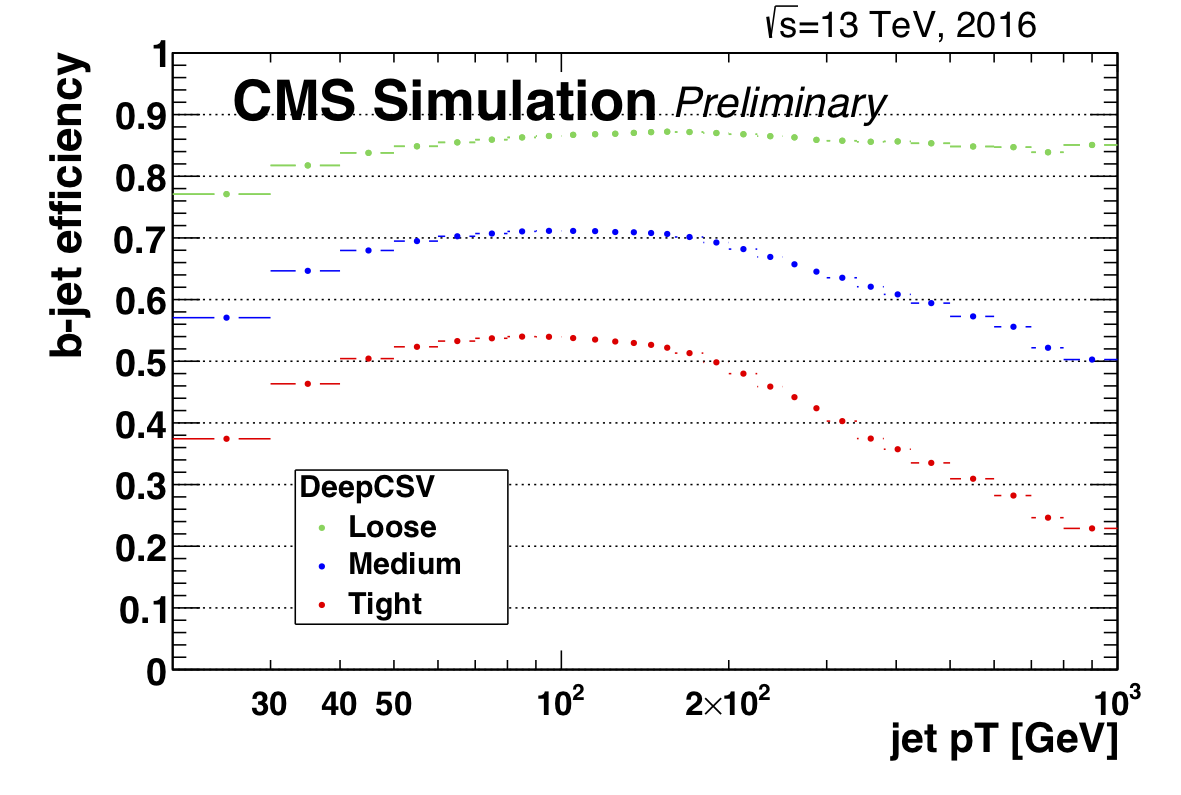
\includegraphics[width=0.75\textwidth]{figures/effvspt_b_deep.png}
 	\singlespace
 	\caption{b-jet efficiency as a function of jet $p_{T}$ for the DeepCSV algorithm. \cite{Sirunyan_2018}}
 \end{figure}

\section{Event Generation}
Searching for new physics can basically be reduced to a search for deviations from the SM. For this reason, extremely accurate signal and SM background predictions are required. For a given analysis, these predictions take the form of samples of events representing various physics scenarios, as they would be seen in the CMS detector. Monte Carlo (MC) event generators are used to simulate proton-proton collisions resulting in a variety of final states. The passage of these final states through the CMS detector is then simulated, and the resulting detector level data is analyzed. The reconstruction algorithms described in the previous section are then run on the simulated data, allowing for a direct comparison with real data.

\subsection{Event Generators}
Event generators are software packages which take as input a desired initial state and simulate all possible outcomes, or a selected subset of outcomes, from an interaction between the specified initial state particles. Bare partons produced in the hard scattering undergo gluon radiation or splitting, and subsequently undergo hadronization to form colorless hadrons. Unstable particle produced in the hard interaction or parton shower are made to decay to stable particles according to their known, or imposed, branching fractions and lifetimes.

During the event generation process, partons which take part in hard scattering interactions with large momentum transfer can be considered free due to asymptotic freedom. The large energy scale involved allows treatment of the interaction using perturbative methods. Under these assumptions, the proton-proton cross section at the LHC for a given $N$ particle final state is given by

\begin{equation}
\sigma_{N} = \sum_{a,b}\int_{0}^{1}dx_{1}\int_{0}^{1}dx_{2}f_{a}(x_{1},\mu^{2})f_{b}(x_{2},\mu^{2})\hat{\sigma}_{N}^{ab}
\end{equation}

where the sum is over all parton species $a$ and $b$ within protons 1 and 2. $f_{i}(x_{j},\mu^{2})$ is the probability (calculated at renormalization scale $\mu^{2}$) of finding parton species $i$ carrying a momentum fraction $x_{j}$ of the parent proton $j$, and $\hat{\sigma}_{N}^{ab}$ is the partonic cross section for initial state $a+b$. The function $f_{i}(x_{j},\mu^{2})$ is referred to as a parton distribution function (PDF). The main task involved in simulation of the hard interaction is the evaluation of this integral. The partonic cross section is itself given by

\begin{equation}
\begin{split}\label{eq:event_generation_partonic_cross_section}
\hat{\sigma}_{N}^{ab}=\int_{cuts}d\hat{\sigma}_{N}^{ab}={}&\frac{\left(2\pi\right)^{4}S}{4\sqrt{\left(p_{1}{\cdot}p_{2}\right)^{2}-m_{1}^{2}m_{2}^{2}}}\times \\ &\int_{cuts} \left[\prod_{i=1}^{N}\frac{d^{3}q_{i}}{\left(2\pi\right)^{3}2E_{i}}\right]\delta^{4}\left(p_{1}+p_{2}-\sum_{i}^{N}q_{i}\right)|\mathcal{M}_{p_{1}p_{2}\rightarrow\{\vec{q}\}}^{ab}|^{2}
\end{split}
\end{equation}

where $p_{i}$ are the incoming particle four-momenta, $q_{i}(E_{i})$ are the outgoing particle four-momenta, $S$ is a product of factors $1/j!$ for each set of $j$ identical particles in the final state, and $\mathcal{M}_{p_{1}p_{2}\rightarrow\{\vec{q}\}}^{ab}$ is the parton level matrix element (ME) for the process. The event generator must build and evaluate all Feynman diagrams associated with the given process to determine the parton level ME, or these must be hard-coded by the package authors. 

The number of diagrams is directly proportional to the final state multiplicity and therefore becomes a complex problem very quickly. Next-to-leading-order (NLO) generators have recently been developed which include loop diagrams. This inclusion complicates the matter enormously as divergences arise in real and virtual contributions which must cancel. 

Once the MEs have been evaluated, the evaluation of the multidimensional phase space integration required for the random sampling is performed using MC techniques. The spectator partons which did not take part in the initial hard interaction can undergo semi-hard interactions with each other, which is referred to as the underlying event (UE). Because these spectator interactions are typically soft, they are not calculable by perturbative methods and empirical models are used to describe them.

Bare partons may be produced as a result of the hard interaction. These partons are perturbatively evolved from the scale of the hard interaction through successive branchings down to a lower energy scale at which they combine to form colorless hadrons, the hadronization scale. These successive branchings are the origin of hadronic jets, whereby individual partons lead to a cascade of partons moving in the general direction of the original parton and sharing its momentum. The probability for a parton to branch into two partons as it evolves from scale $t$ to $t'<t$ and the kinematics of such a branching can ce calculated form first principles, accurate to fixed order in the strong coupling; the results of which are known as the DGLAP evolution equations. Thus, the partons are recursively evolved down to the hadronization scale through successive branchings. Care must be taken to avoid double counting of regions in phase-space. After showering of an N-1 particle final state, an additional hard parton can be radiated, thus producing overlap with an $N$ particle interaction hard state. The colored proton remnants which did not take part in the hard interaction can produce showers as well. 

At the hadronization scale, the showering ceases and the colored partons group to form colorless hadrons. This regime is not amenable to perturbative calculations, and no first-principle theory is viable. Various phenomenological methods have been developed to model hadronization, including the \textit{Lund-string-model} and the \textit{cluster hadronization model}. In the Lund model, color string attach to a pair of quarks, and as these strings stretch, energy is built up in the electromagnetic field until vacuum excitation of a quark-antiquark pair becomes possible. Ultimately, color connected pairs of quarks form hadrons. 

The cluster hadronization model assumes a local parton-hadron duality, this hadronic quantum numbers result from the quantum numbers of local partons with minimal disruption needed to produce colorless hadrons. Regardless of the hadronization model choice, the produced hadrons are often unstable, and are then decayed to stable hadrons.

\subsubsection{Pythia}

PYTHIA is a general purpose, tree level partonic ME generator capable of performing parton showering, hadronization, and UE simulation. A variety of $2\rightarrow1,2,3$ processes are included. Full spin correlations are included in the decays of unstable resonances. Shower evolution proceeds in terms of decreasing time-like virtuality, and imposes angular ordering by veto. Shower evolution is accurate to the LL level. The Lund string model is used for hadronization. UE interactions are described perturbatively as multiple nearly-independent $2\rightarrow 2$ scatterings. PYTHIA 8 is used in this analysis to simulate signal samples with $xqcut=30$ and $qcut=60$.

\subsubsection{MADGRAPH}

MADGRAPH is another generator that is used in this analysis for simulating hard parton emission (ie. ISR and FSR), but must be interfaced with PYTHIA for showering and collinear radiation.

\subsection{Detector Simulation}

The next step in the simulation of events chain is the simulation of how particles will interact with the detector and its constituent materials or how the readout electronics will behave. To simulate the response of the CMS detector, the generators are interfaced with a sophisticated detector simulation based on the GEANT4 software package, which takes into account the exact detector geometry as well as all materials used.

The alignment, calibration, and other conditions which may change over time are periodically checked and stored in a database. These conditions are used for both offline simulation and reconstruction as well as for online activities. A snapshot of the conditions at some point in time is called a global tag. For reference, this analysis uses the $80X\_dataRun2\_2016LegacyRepro\_v4$ and $80X\_mcRun2\_asymptotic\_2016\_TrancheIV\_v8$ global tags for data and simulation, respectively. 

The final state particles from the event generator are sent to the detector simulation, which tracks the particles as they move through the detector depositing energy into what are called simulated hits. While the models of electromagnetic interactions are extremely precise, the hadronic interactions have a greater uncertainty associated with them. The simulation goes through the data acquisition process, event simulating the responses of the photodetectors and readout electronics. The resulting information is then analyzed by the same reconstruction process that the real data goes through and is stored using the ROOT software library. 

